\chapter{夫琅禾费衍射与空间滤波}\label{ch:b2:diffraction}

透过两根手指之间的缝隙眯眼看街灯，
灯光便拉成一条条条纹；
用最精细的望远镜观察恒星，看到的并不是一个点，而是一个小圆盘，
外围环绕着若隐若现的圆环。光穿过开口便会扩散——
开口越窄，扩散越宽——任何透镜都无法把光
聚得比这种扩散所允许的更细。这就是\emph{衍射}，
它使显微镜看不清病毒，望远镜的分辨本领
随口径增大而提高，激光束也无法保持平行。本章
计算远场中孔径的衍射图样，
它对每一台光学仪器施加的极限，它与
干涉的结合方式，以及阿贝的思想——把透镜的焦平面
变成一个可对像进行滤波的场所。

\section{惠更斯–菲涅耳原理与夫琅禾费区}

\begin{definition}[惠更斯–菲涅耳原理]\label{def:b2:diffraction:huygens}
\index{惠更斯–菲涅耳原理}\index{衍射}\index{夫琅禾费衍射}
波前上的每一点（或被波照亮的孔径上的每一点）都充当次级波源，
发出球面子波，其相位与该处的波一致；
其后方的波是这些子波的相干叠加。对被平面波照亮的孔径 $\Sigma$，
设其振幅为 $a$，则到达远处一点的振幅为
$\underline s(M) = K\iint_\Sigma\eu^{-\iu\varphi(P, M)}\dd S$，其中
$\varphi(P, M)$ 为从孔径上的点 $P$ 到 $M$ 的路径相位，
$K$ 为常数。\emph{夫琅禾费}（远场）衍射是指 $M$ 位于无穷远处——或位于透镜的焦平面上——的情形，
此时从孔径各点射向 $M$ 的光线
彼此平行，
方向为 $\vect u$，且
\[
\varphi(P, M) = \varphi_0 - \frac{2\pi}\lambda\,\vect{OP}\cdot\vect u , \qquad
\underline s(\vect u) \propto \iint_\Sigma\eu^{\iu(2\pi/\lambda)\vect{OP}\cdot\vect u}\dd S .
\]
衍射图样在无穷远处观察，或在透镜的焦点 $F'$ 处观察，
此时方向为 $\vect u$、夹角为小角度 $(\alpha, \beta)$ 的光线映射到
点 $(f\alpha, f\beta)$。
\end{definition}
\admitted

\begin{remark}[距离多远才算足够远？]\label{rem:b2:diffraction:fresnelnumber}
\index{菲涅耳数}
对尺寸为 $D$ 的孔径，在不用透镜、距离为 $L$ 处观察时，
要使光线足够平行，需要 \cref{exo:b2:scalar-light-model:12} 中的二次项
可以忽略，$D^2/L \ll \lambda$——
也就是\emph{菲涅耳数} $D^2/\lambda L \ll 1$。宽 \qty{0.1}{mm} 的狭缝
在 \qty{500}{nm} 光照下需要 $L \gg \qty{2}{cm}$；直径 \qty{1}{cm} 的孔径则需要 $L \gg \qty{200}{m}$——
因此要借助透镜，它把无穷远处映射到焦平面上。较近时
属于菲涅耳衍射，图样更为复杂；
例如直边的阴影在亮的一侧会出现条纹。
\end{remark}

\section{单缝与圆孔}

\begin{proposition}[单缝衍射]\label{prop:b2:diffraction:slit}
\index{单缝衍射}\index{sinc 函数}
宽为 $b$（沿 $y$ 方向很长）的狭缝在垂直入射下，
在方向 $\theta$（垂直于狭缝的平面内）上的
光强为
\[
I(\theta) = I_0\,\operatorname{sinc}^2\Bigl(\frac{\pi b\sin\theta}\lambda\Bigr) , \qquad \operatorname{sinc}x = \frac{\sin x}x :
\]
中央亮纹的角半宽为 $\lambda/b$（第一零点位于
$\sin\theta = \pm\lambda/b$），包含 $90\%$ 的光能；次极大位于
约 $\sin\theta = \pm1.43\lambda/b$、$\pm2.46\lambda/b$、\dots 处，
其相对光强分别为 $4.7\%$、$1.6\%$、\dots——缝越窄，图样越宽。
在焦距为 $f$ 的透镜焦平面上，
中央亮纹的宽度为 $2\lambda f/b$。
\end{proposition}

\begin{proof}
$\underline s(\theta) \propto \int_{-b/2}^{b/2}\eu^{\iu kx\sin\theta}\dd x = b\,\operatorname{sinc}(kb\sin\theta/2)$
其中 $k = 2\pi/\lambda$；取模平方即得光强。当 $b\sin\theta = m\lambda$，$m \ne 0$ 时
为零点：此时狭缝两半边发出的子波两两相消。
\end{proof}

\begin{omfigure}
\begin{tikzpicture}[font=\small, x=1cm, y=1cm, >=Stealth]
  \begin{scope}
    \draw[thick] (0,-2) -- (0,-0.5) (0,0.5) -- (0,2);
    \draw[<->] (-0.35,-0.5) -- (-0.35,0.5) node[midway, left, font=\footnotesize] {$b$};
    \foreach \y in {-1.6,-0.9,-0.2,0.5,1.2} \draw[omDef, ->] (-2.2,\y) -- (-0.1,\y);
    \foreach \y in {-0.4,-0.2,0,0.2,0.4} \draw[omThm, thick, ->] (0.1,\y) -- (2.4,{\y+1.0});
    \draw[dashed] (0.1,0) -- (2.6,0); \draw (1.4,0) arc[start angle=0, end angle=23.5, radius=1.4]; \node[font=\footnotesize] at (1.7,0.28) {$\theta$};
    \node[font=\footnotesize] at (1.2,-1.6) {$b\sin\theta = \lambda$：第一零点};
  \end{scope}
  \begin{scope}[xshift=8.6cm]
    \begin{axis}[omaxis, axis x line=bottom, axis y line=left, width=6.4cm, height=4.4cm, at={(0,-2.0cm)},
        xlabel={$b\sin\theta/\lambda$}, ylabel={$I/I_0$}, xmin=-3.2, xmax=3.2, ymin=0, ymax=1.1, xtick={-3,-2,-1,0,1,2,3}, ytick={0.5,1}, samples=400,
        xlabel style={at={(axis description cs:0.5,-0.14)}, anchor=north},
        ylabel style={at={(axis description cs:-0.1,0.5)}, rotate=90, anchor=south}]
      \addplot[omDef, thick, domain=-3.2:3.2] {(sin(deg(pi*x))/(pi*x+1e-9))^2};
    \end{axis}
  \end{scope}
\end{tikzpicture}

{\small 左：狭缝两侧的子波在方向
$\theta$ 上的叠加。右：狭缝的夫琅禾费图样，即 $\operatorname{sinc}^2$：
中央瓣的宽度为其他瓣的两倍，且亮得多。}
\end{omfigure}

\begin{proposition}[圆孔衍射；艾里斑]\label{prop:b2:diffraction:airy}
\index{艾里斑}\index{瑞利判据（分辨）}\index{分辨本领（仪器）}
直径为 $D$ 的圆孔产生一个中央亮斑，
即\emph{艾里斑}，其外围环绕着若隐若现的圆环；第一个暗环位于
\[
\sin\theta = 1.22\,\frac\lambda D ,
\]
艾里斑内集中了 $84\%$ 的光能。任何入瞳直径为 $D$ 的仪器——
眼睛、照相机、望远镜、显微镜物镜——
都会把点光源成像为角半径如上的艾里斑；
若两点可被\emph{分辨}（瑞利判据），即角间距超过
$1.22\lambda/D$ 时，
此角间距即仪器的分辨本领。
\end{proposition}
\admitted

\begin{example}[眼睛、望远镜、显微镜]\label{ex:b2:diffraction:instruments}
眼睛（$D = \qty{3}{mm}$，$\lambda = \qty{550}{nm}$）：$1.22\lambda/D = \qty{2.2e-4}{rad}$，约
\qty{45}{''}——在 \qty{4}{m} 处可分辨 \qty{1}{mm} 的细节，这大致就是
优秀眼睛的视力：进化使视网膜细胞与
衍射极限相匹配。口径 \qty{2.4}{m} 的望远镜：\qty{0.06}{''}，好了约一千倍，
前提是大气允许（地面上并非如此：
\qty{1}{''} 的“视宁度”所限，因此才有太空望远镜与自适应光学）。
口径 \qty{100}{m} 的射电天线，$\lambda = \qty{21}{cm}$：\qty{9}{'}，比眼睛还差；
跨越大陆的干涉仪恢复了分辨本领。
孔径角为 $\alpha$ 的显微镜物镜，可分辨的最小距离为 $0.61\lambda/n\sin\alpha$
——在可见光中约为 \qty{0.2}{\micro m}，与放大倍数无关：这一极限
促使显微术转向电子与 X 射线。
\end{example}

\begin{omfigure}
\begin{tikzpicture}[font=\small, x=1cm, y=1cm]
  \begin{scope}
    \foreach \r/\g in {1.5/85, 1.25/70, 1.0/50, 0.8/25, 0.6/5, 0.45/40, 0.3/70, 0.15/95} {
      \fill[black!\g] (0,0) circle (\r);
    }
    \node[font=\footnotesize] at (0,-1.9) {单颗恒星的艾里斑};
  \end{scope}
  \begin{scope}[xshift=4.2cm]
    \foreach \r/\g in {0.8/25, 0.6/5, 0.45/40, 0.3/70, 0.15/95} {
      \fill[black!\g] (-0.45,0) circle (\r);
    }
    \foreach \r/\g in {0.8/25, 0.6/5, 0.45/40, 0.3/70, 0.15/95} {
      \fill[black!\g, opacity=0.6] (0.45,0) circle (\r);
    }
    \node[font=\footnotesize] at (0,-1.9) {瑞利极限下的两颗恒星};
  \end{scope}
  \begin{scope}[xshift=9.6cm]
    \begin{axis}[omaxis, axis x line=bottom, axis y line=left, width=5.4cm, height=4.0cm, at={(0,-1.8cm)},
        xlabel={$\theta D/\lambda$}, ylabel={$I$}, xmin=-2.5, xmax=3.5, ymin=0, ymax=1.5, xtick={-1.22,0,1.22,2.44}, xticklabels={$-1.22$,$0$,$1.22$,$2.44$}, ytick=\empty, samples=300,
        xlabel style={at={(axis description cs:0.5,-0.14)}, anchor=north},
        ylabel style={at={(axis description cs:-0.06,0.5)}, rotate=90, anchor=south}]
      \addplot[omDef, thick, domain=-2.5:3.5] {(sin(deg(pi*x/1.22))/(pi*x/1.22+1e-9))^2};
      \addplot[omThm, thick, domain=-2.5:3.5] {(sin(deg(pi*(x-1.22)/1.22))/(pi*(x-1.22)/1.22+1e-9))^2};
    \end{axis}
  \end{scope}
\end{tikzpicture}

{\small 左图与中图：点光源的艾里斑，以及两个
处于瑞利极限的光源——其中一个的中心位于另一个的第一
暗环上。右图：二者的光强分布（以 $\operatorname{sinc}^2$
形状示意），间距为 $1.22\lambda/D$。}
\end{omfigure}

\section{衍射与干涉的结合}

\begin{proposition}[有限宽的杨氏双缝；光栅的包络]\label{prop:b2:diffraction:combined}
\index{衍射包络}\index{缺级}
缝宽为 $b$、中心间距为 $a$ 的两条狭缝给出
\[
I(\theta) = 4I_0\,\operatorname{sinc}^2\Bigl(\frac{\pi b\sin\theta}\lambda\Bigr)\cos^2\Bigl(\frac{\pi a\sin\theta}\lambda\Bigr) :
\]
杨氏条纹（间距为 $\lambda/a$，按 $\sin\theta$ 计）位于单缝
包络（宽度为 $2\lambda/b$）之下；中央瓣内有 $a/b$ 条条纹，而
满足 $a\sin\theta = p\lambda$、落在包络零点上的条纹，
即 $b\sin\theta = m\lambda$ 处的条纹，是\emph{缺级}。由 $N$ 条缝组成、缝宽为
$b$，其主极大同样受同一包络调制——
在\cref{ch:b2:gratings}中的闪耀使其偏向所用的级次。
\end{proposition}

\begin{proof}
孔径积分可分解为两条缝上同一积分之和，
各积分分别平移 $\pm a/2$：$\underline s \propto b\,\operatorname{sinc}(\pi b\sin\theta/\lambda)
\times2\cos(\pi a\sin\theta/\lambda)$。对于 $N$ 条缝，第二个因子即为
$N$ 波之和。
\end{proof}

\begin{omfigure}
\begin{tikzpicture}
\begin{axis}[omaxis, axis x line=bottom, axis y line=left, width=13.6cm, height=4.6cm,
    xlabel={$a\sin\theta/\lambda$}, ylabel={$I/4I_0$}, xmin=-9, xmax=9, ymin=0, ymax=1.1, xtick={-8,-4,0,4,8}, ytick={0.5,1}, samples=1200,
    xlabel style={at={(axis description cs:0.5,-0.12)}, anchor=north},
    ylabel style={at={(axis description cs:-0.04,0.5)}, rotate=90, anchor=south}]
  \addplot[omDef, thick, domain=-9:9] {(sin(deg(pi*x/4))/(pi*x/4+1e-9))^2*cos(deg(pi*x))^2};
  \addplot[omThm, thick, dashed, domain=-9:9] {(sin(deg(pi*x/4))/(pi*x/4+1e-9))^2};
\end{axis}
\end{tikzpicture}

{\small 两条缝，$a = 4b$：杨氏条纹位于单缝
包络（虚线）之下；第四级条纹落在
包络零点上，因而缺失。}
\end{omfigure}

\section{傅里叶平面与空间滤波}

\begin{proposition}[作为傅里叶分析器的透镜]\label{prop:b2:diffraction:fourier}
\index{傅里叶平面}\index{空间频率}\index{空间滤波}\index{阿贝显微成像理论}
透射率为 $t(x, y)$ 的透明片位于透镜的前焦面上，
由平面波照明，则在后焦面上得到
振幅
\[
\underline s(X, Y) \propto \iint t(x, y)\,\eu^{-\iu2\pi(xX + yY)/\lambda f}\dd x\,\dd y
\]
——即其二维傅里叶变换，\emph{傅里叶平面}上的每一点 $(X, Y)$
收集沿角度
$(X/f, Y/f)$ 衍射的光，即物体的\emph{空间频率} $(X/\lambda f, Y/\lambda f)$：
远离轴处为精细细节（高频），靠近轴处则为粗略结构
（低频）。第二块透镜由该平面重新成像，凡在该平面上
被挡住或改变的部分，都会从像中滤除
（\emph{空间滤波}，阿贝显微成像理论）：
轴上的针孔只保留低频（平滑，“净化”
激光束）；轴上的挡板去除均匀背景，
保留边缘（暗场法、纹影法）；轴上的四分之一波片
使原本不可见的相位物体转化为强度对比
（相衬法，泽尼克）。
\end{proposition}

\begin{proof}[说明]
在夫琅禾费积分中，$\vect{OP}\cdot\vect u = x\alpha + y\beta$，
方向映射为 $(X, Y) = (f\alpha, f\beta)$；透射率给出各次级波源的权重。
（傅里叶变换本身将在
本科三年级数学分册中研究；此处它只是这一积分的名称。）
对周期为 $d$ 的周期物体，其变换是一组光栅
级次，位于 $X = p\lambda f/d$ 处：像要能显示周期，至少
须让级次 $\pm1$ 通过透镜——这就是阿贝条件，
亦即显微镜分辨极限的再次体现。
\end{proof}

\begin{omfigure}
\begin{tikzpicture}[font=\small, x=1cm, y=1cm, >=Stealth]
  \draw[omDef, thick, ->] (-5.6,0.8) -- (-4.6,0.8); \draw[omDef, thick, ->] (-5.6,0) -- (-4.6,0); \draw[omDef, thick, ->] (-5.6,-0.8) -- (-4.6,-0.8);
  \draw[thick, fill=omExo!20] (-4.4,-1.4) rectangle (-4.3,1.4); \node[font=\footnotesize] at (-4.35,-1.75) {物体 $t(x, y)$};
  \draw[thick, fill=omExo!20] (-2.4,0) ellipse (0.2 and 1.5); \node[font=\footnotesize] at (-2.4,-1.85) {$L_1$};
  \draw[thick] (0,-1.4) -- (0,1.4); \fill[omThm] (0,0) circle (2pt); \fill[omThm] (0,0.7) circle (1.5pt); \fill[omThm] (0,-0.7) circle (1.5pt);
  \node[font=\footnotesize] at (0,-1.75) {傅里叶面};
  \draw[thick, fill=omExo!20] (2.4,0) ellipse (0.2 and 1.5); \node[font=\footnotesize] at (2.4,-1.85) {$L_2$};
  \draw[thick, fill=omExo!20] (4.3,-1.4) rectangle (4.4,1.4); \node[font=\footnotesize] at (4.35,-1.75) {像};
  \draw[omThm] (-4.35,0.6) -- (-2.4,1.0) -- (0,0.7) -- (2.4,0.4) -- (4.35,-0.6);
  \draw[omThm] (-4.35,-0.6) -- (-2.4,-1.0) -- (0,-0.7) -- (2.4,-0.4) -- (4.35,0.6);
  \draw[omProp] (-4.35,0.6) -- (-2.4,0.6) -- (0,0) -- (2.4,-0.6) -- (4.35,-0.6);
  \draw[omProp] (-4.35,-0.6) -- (-2.4,-0.6) -- (0,0) -- (2.4,0.6) -- (4.35,0.6);
  \draw[<->] (-4.35,1.7) -- (-2.4,1.7) node[midway, above, font=\footnotesize] {$f$}; \draw[<->] (-2.4,1.7) -- (0,1.7) node[midway, above, font=\footnotesize] {$f$};
  \node[omThm, font=\footnotesize, anchor=west] at (0.15,0.95) {周期物体的级次};
\end{tikzpicture}

{\small $4f$ 装置：第一块透镜在其焦面上形成物体的
傅里叶变换（周期物体在此处给出分立的级次），
第二块透镜重新成像；傅里叶面上的
掩模对像进行滤波。}
\end{omfigure}

\begin{example}[清洁光束，看见不可见之物]\label{ex:b2:diffraction:filtering}
激光束携带尘埃与起伏的扰动：将其聚焦通过一个
几微米的针孔——与洁净高斯光束中央艾里斑的大小相当——
其余位于外侧的一切均被挡去；
重新准直后的光束变得平滑，这就是\emph{空间滤波器}。活
细胞是透明的，它只改变光的相位。挡住
轴上斑点使其边缘在黑底上发亮；泽尼克的
板将未衍射的光移动四分之一波长，使其与衍射光
在强度上干涉：细胞内部得以显现，
生物学由此获得了它的显微镜（1953 年诺贝尔奖）。
\end{example}

\begin{method}[衍射的数量估算]\label{met:b2:diffraction:method}
(1) 角展宽 $\sim\lambda/b$，孔径尺寸为 $b$（
圆孔为 $1.22\lambda/D$）；图样在距离 $L$ 处或焦距 $f$ 时的大小为
$\lambda L/b$、$\lambda f/b$。(2) 检验夫琅禾费条件 $b^2/\lambda L \ll 1$，或
使用透镜。(3) 综合：衍射包络 $\times$ 干涉
条纹。(4) 分辨：两点需 $\Delta\theta > 1.22\lambda/D$；周期
物体需要其一级次进入光瞳。(5) 傅里叶面的图像：
挡去什么即可去掉哪种细节。
\end{method}

\section{练习}

\begin{exercise}[$\star$]\label{exo:b2:diffraction:1}
用氦氖激光器（\qty{633}{nm}）照亮宽 \qty{0.10}{mm} 的单缝；屏幕位于
\qty{2.0}{m} 处，求中央极大的宽度与前两个次极大的位置；
并求菲涅耳数——屏幕是否足够远？再考虑
同一单缝配以 $f = \qty{50}{cm}$ 的透镜时的情形。
\end{exercise}

\begin{exercise}[$\star$]\label{exo:b2:diffraction:2}
求下列各者的分辨本领（瑞利判据）：人眼（\qty{3}{mm}，\qty{550}{nm}）；一
\qty{10}{cm} 的业余望远镜；\qty{2.4}{m} 的哈勃望远镜主镜；\qty{64}{m} 的
射电天线，波长 \qty{6}{cm}；\qty{50}{mm} 照相机镜头，$f/8$（光瞳 \qty{6}{mm}）：
求感光元件上艾里斑的大小，并与 \qty{4}{\micro m} 的像素相比较。
\end{exercise}

\begin{exercise}[$\star$]\label{exo:b2:diffraction:3}
两缝宽 $b = \qty{0.05}{mm}$，中心相距 $a = \qty{0.25}{mm}$，$\lambda =
\qty{500}{nm}$，透镜 $f = \qty{1}{m}$：求条纹间距；中央
包络的宽度；其中的条纹数；哪些级次缺失？
\end{exercise}

\begin{exercise}[$\star$]\label{exo:b2:diffraction:4}
一束直径 \qty{2}{mm}、波长 \qty{633}{nm} 的激光束传播至月球（
距离 \qty{3.8e8}{m}）：衍射角 $\sim1.22\lambda/D$，光斑直径；
以 \qty{3.5}{m} 望远镜作发射器；为何月球激光测距的回波如此
微弱（角反射器，\qty{1}{m}，以自身的
衍射将光送回）？
\end{exercise}

\begin{exercise}[$\star\star$]\label{exo:b2:diffraction:5}
\emph{单缝细究。}(a) 对单缝作夫琅禾费积分，
并得到 $\operatorname{sinc}^2$。(b) 证明次极大
位于 $\tan x = x$（$x = \pi b\sin\theta/\lambda$）处，第一个在 $x = 1.43\pi$ 附近，并
计算其相对强度。(c) 中央瓣所占能量的比例
（可取 $\int_{-\pi}^\pi\operatorname{sinc}^2 = 0.903\pi$ 及
$\int_{-\infty}^\infty\operatorname{sinc}^2 = \pi$）。(d) 单缝以入射角
$\theta_0$ 照明，证明图样形状不变，中心位于方向 $\theta_0$ 上。
\end{exercise}

\begin{exercise}[$\star\star$]\label{exo:b2:diffraction:6}
\emph{显微镜。}数值孔径为 $n\sin\alpha = 1.4$ 的物镜
（油浸）在 \qty{500}{nm} 下：最小可分辨距离 $0.61\lambda/n\sin
\alpha$；换用蓝光（\qty{400}{nm}）时；紫外（\qty{250}{nm}）时；为何
$1000\times$ 的目镜无济于事（人眼在 \qty{25}{cm} 处的
极限为 \qty{0.1}{mm}）？电子显微镜改变了什么（$\lambda = \qty{4}{pm}$，
\qty{100}{keV}）？
\end{exercise}

\begin{exercise}[$\star\star$]\label{exo:b2:diffraction:7}
\emph{矩形与圆形。}(a) 矩形孔径 $b \times h$：
证明图样为 $\operatorname{sinc}^2(\pi b\sin\theta_x/\lambda)\operatorname{sinc}^2(\pi h
\sin\theta_y/\lambda)$，呈十字形，且沿较窄一边的方向更宽。(b) 边长为
\qty{0.2}{mm} 的正方形孔径，$f = \qty{1}{m}$：求中央正方形的大小。(c) 对
同样宽度的圆孔，第一零点位于 $1.22\lambda/D$ 而非 $\lambda/b$：
为何更远？（想一想：光集中在圆盘的
中心附近）？(d) 望远镜的次镜由四根支杆固定：它们
会给亮星的像添加什么？
\end{exercise}

\begin{exercise}[$\star\star$]\label{exo:b2:diffraction:8}
\emph{阿贝。}一块周期为 $d = \qty{2}{\micro m}$ 的光栅，用
孔径角为 $\alpha$、置于空气中的显微物镜观察，$\lambda = \qty{550}{nm}$。
(a) 求其 $\pm1$、$\pm2$ 级的衍射角。(b) 为使像能显示周期，
$\sin\alpha$ 的最小值为多少（$\pm1$ 级必须进入物镜）。(c) 取 $\sin\alpha = 0.4$：像呈现什么？
——它是否忠实地反映光栅？(d) 斜入射照明使零级与
\emph{一}个一级衍射光通过，此时
$\sin\alpha$ 的最小值及增益为多少。
\end{exercise}

\begin{exercise}[$\star\star$]\label{exo:b2:diffraction:9}
\emph{空间滤波器。}一束直径为 \qty{2}{mm} 的激光束（$\lambda = \qty{633}{nm}$）经
焦距为 $f = \qty{20}{mm}$ 的透镜聚焦，穿过一针孔。(a) 焦平面上
中央艾里斑的直径；使其通过的针孔直径（取 $1.5\times$）。(b) 光束上一粒
直径为 \qty{50}{\micro m} 的尘埃，其衍射光的角度为多少？
这些光落在焦平面上何处——是否穿过针孔？(c) 若光束为高斯型，
针孔通过其中 $99\%$ 的能量，则损失的功率为多少？
为何出射光束是平滑的？
(d) 为何针孔必须对中到
几微米的精度？
\end{exercise}

\begin{exercise}[$\star\star\star$]\label{exo:b2:diffraction:10}
\emph{巴比涅。}两块互补的屏（一条狭缝，以及一条同宽的
不透明条带）由平面波照明。(a) 证明：在偏离入射光方向处，
二者的夫琅禾费图样相同（两振幅之和等于无遮挡波的振幅，
轴外为零）。(b) 用激光照射直径为
\qty{80}{\micro m} 的毛发，距离 \qty{2}{m}，求其图样的条纹间距，
并由此求出毛发的直径——这是一种标准测量。
(c) 轴上本身会看到什么？
(d) 薄云中的小液滴为何
会在月球周围形成彩色光环，
光环的半径给出什么？
\end{exercise}

\begin{exercise}[$\star\star\star$]\label{exo:b2:diffraction:11}
\emph{暗场与相位衬度。}一个透明物体，其
透射函数 $t(x) = \eu^{\iu\varphi(x)} \approx 1 + \iu\varphi(x)$，其中 $|\varphi| \ll 1$。(a) 其普通像的
强度：证明它在一阶近似下是均匀的——不可见。(b)
在傅里叶面上，“1”是轴上斑点，$\iu\varphi$ 是其周围的衍射光：
若挡板遮住轴上斑点，则像的
强度 $\propto\varphi^2$——暗场，其弱点在于光弱。(c) 若改为轴上斑点
延迟 $\pi/2$（乘以 $\iu$），则像的强度 $\propto|1 +
\varphi|^2 \approx 1 + 2\varphi$——相位衬度，与 $\varphi$ 呈线性关系。(d) 为何泽尼克板
往往也是吸收性的（它会衰减轴上斑点）？
\end{exercise}

\begin{exercise}[$\star\star\star$]\label{exo:b2:diffraction:12}
\emph{光谱仪狭缝像与光栅的分辨本领。}一块宽度为
$W$ 的光栅即光谱仪的孔径：证明该孔径的
衍射图样 $\operatorname{sinc}^2(\pi W\sin\theta/\lambda)$
（对于 $\theta \approx 0$ 方向射出的光束）的角半宽度为
$\lambda/W$，并通过色散 $p/a\cos
\theta$ 换算为波长，即 $\Delta\lambda = \lambda/pN$——此即
在\cref{ch:b2:gratings}中所述的分辨本领，从衍射角度看。(b) 一台口径为
$D$ 的望远镜与宽度为 $W$ 的光栅：光栅必须宽于
$D\,f_{\text{准直}}/f_{\text{望远}}$，为什么？(c) 用一句话说明为何
光学中每一种“分辨本领”均为 $\sim$（孔径尺寸）/$\lambda$。
(d) 狭缝带来什么影响？它何时起主导作用？
\end{exercise}

\begin{omfigure}
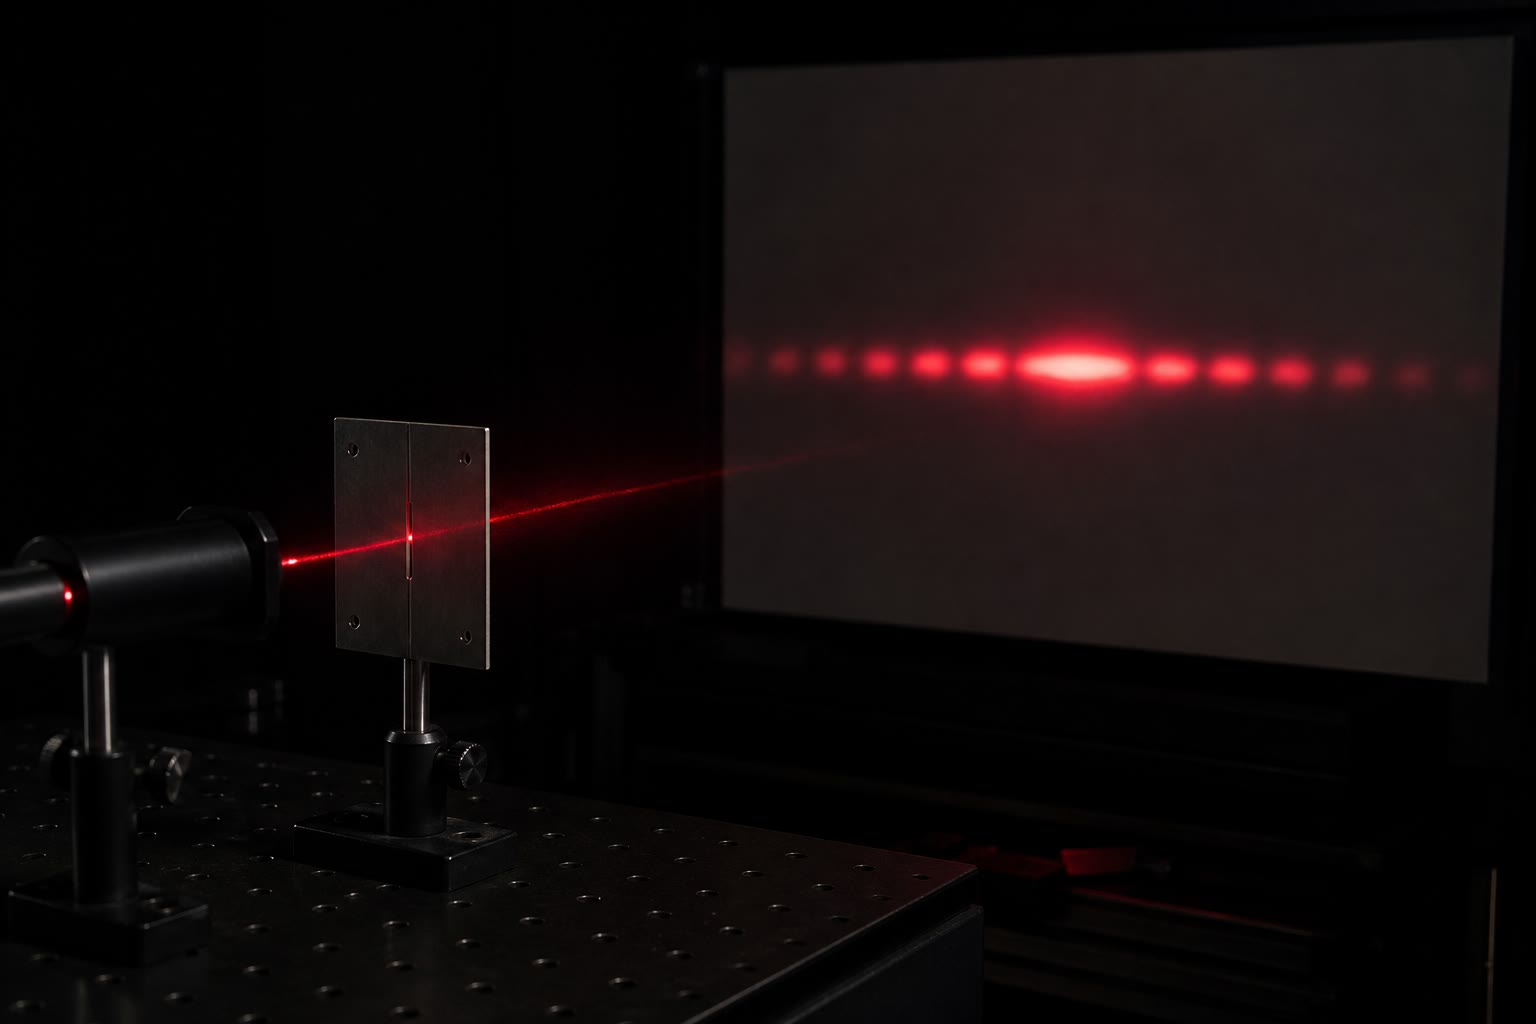
\includegraphics[width=0.58\linewidth]{images/book4/ai/b4-22-slit-diffraction-pattern.jpg}

{\small 激光束通过一狭缝：在远处的屏上，可见宽亮的中央亮带，以及夫琅禾费图样中较弱、较窄的两侧次极大。}
\end{omfigure}

\section{问题：可分辨什么}

\begin{problem}[{周末问题——四个尺度上的衍射极限：
眼睛、望远镜、显微镜，以及必须在使用前先清理的
激光束}]
\label{pb:b2:diffraction:1}

\medskip
\noindent\textbf{第一部分——眼睛。}
白天瞳孔直径 $D = \qty{3}{mm}$，夜晚为 \qty{7}{mm}；$\lambda = \qty{550}{nm}$；
视网膜中央凹处视锥细胞的间距为 \qty{2}{\micro m}，眼睛的
焦距为 \qty{17}{mm}。
\begin{enumerate}
  \item 白天艾里斑的角半径；其在
        视网膜上的线半径；与视锥间距比较——
        视网膜是否与光学系统匹配？
  \item 在 \qty{25}{cm} 处能分辨的两点最小间距；在
        \qty{10}{m} 处呢？在手臂长的距离处能否辨认 \qty{1}{mm} 的字？
  \item 夜晚瞳孔开大至 \qty{7}{mm}：此时的衍射极限为多少；
        为何视力仍会变差（全孔径下透镜的像差，
        视杆细胞比视锥细胞粗）？
  \item 两盏车前灯相距 \qty{1.5}{m}，在
        多远处它们会合并为一盏灯？
  \item 将一个 \qty{1}{mm} 的小孔置于眼前：衍射会产生什么效果；
        为何针孔仍能帮助近视的眼睛
        （景深）？
\end{enumerate}

\medskip
\noindent\textbf{第二部分——望远镜。}
一台 \qty{1}{m} 口径的望远镜，$f = \qty{10}{m}$，配有像元为
\qty{10}{\micro m} 的照相机；$\lambda = \qty{550}{nm}$。
\begin{enumerate}[resume]
  \item 以角秒计的衍射极限；探测器上艾里斑的半径；
        每个艾里斑占的像元数。
  \item 大气将像模糊至 \qty{1}{''}，
        望远镜的分辨本领损失了多少？使衍射极限
        恰等于视宁度的望远镜口径为多大？
  \item 自适应光学在 \qty{2.2}{\micro m} 处校正大气：此处的衍射极限为多少；
        为何在红外更容易实现？
  \item 一对双星的两子星相距 \qty{0.15}{''}：能否用 \qty{2.2}{\micro m}
        的自适应光学分辨？在太空中以 \qty{550}{nm} 的波长呢？
  \item 月球距离为 \qty{3.8e5}{km}：此望远镜能分辨的最小环形山
        （仅考虑衍射）为多大；月球着陆器的足迹
        （\qty{4}{m}）又为多大？
  \item 望远镜相对夜晚眼睛（\qty{7}{mm}）的集光本领为多少；
        这带来了什么好处，又不能带来什么？
  \item 一颗恒星的光穿过固定次镜的四根支杆，
        描述所成的像。
\end{enumerate}

\medskip
\noindent\textbf{第三部分——显微镜。}
物镜的数值孔径 $\mathrm{NA} = n\sin\alpha = 0.9$（干式）或 $1.4$
（油浸），$\lambda = \qty{550}{nm}$；可分辨距离为 $0.61\lambda/\mathrm{NA}$。
\begin{enumerate}[resume]
  \item 各物镜的可分辨距离；
        以及每毫米内的线对数。
  \item 一个 \qty{1}{\micro m} 的细菌，其内部结构尺度为 \qty{0.2}{\micro m}：
        两种物镜各能看到什么？一个 \qty{0.1}{\micro m} 的病毒呢？
  \item 阿贝判据：周期为 $d$ 的周期结构，只有其
        在 $\sin\theta = \lambda/d$ 处的一级衍射进入物镜时才能成像：求最小的 $d$，
        设 $\mathrm{NA} = 1.4$，并与 $0.61\lambda/\mathrm{NA}$ 比较。
  \item 为何载玻片与物镜之间加油能提高
        分辨率？
  \item 波长 \qty{250}{nm} 的紫外光与电子显微镜（取波长 \qty{4}{pm}）：
        用同一公式比较二者的可分辨距离（对电子，实际数值孔径取
        \qty{0.01}{}）。
  \item 细胞是透明的：在明场下其像是空的。
        请用两句话解释物镜的
        傅里叶面上的相衬板起什么作用。
\end{enumerate}

\medskip
\noindent\textbf{第四部分——光束。}
一台输出波长为 \qty{532}{nm} 的激光器，光束直径为 \qty{1.5}{mm}，
需将其扩束至 \qty{30}{mm} 并加以净化。
\begin{enumerate}[resume]
  \item 原始光束的衍射半角（$\sim1.22\lambda/D$）；
        无光学元件时，经 \qty{100}{m} 后其直径为多少。
  \item 一个焦距 $f_1 = \qty{10}{mm}$ 的透镜将其聚焦：求焦斑直径；
        并选取针孔直径（取为焦斑的 $1.5\times$）。
  \item 第二个焦距为 $f_2$ 的透镜将光束重新准直至 \qty{30}{mm}：求 $f_2$；
        新的衍射角；经 \qty{1}{km} 后的直径。
  \item 第一透镜上 \qty{100}{\micro m} 的灰尘以何角度衍射；
        这部分光落在针孔平面的何处？
        它又会发生什么？
  \item 针孔透过高斯光束的 $99\%$：
        损失的功率及其去向。
  \item 为何扩束后的光束必须\emph{更大}才能保持平行
        （将 $\lambda/D$ 与光束直径翻倍的距离，
        $\sim D^2/\lambda$ 联系起来）？
  \item 用一张表总结本题的四个限制：孔径、波长、
        $\lambda/D$ 及其所限制的对象。
\end{enumerate}
\end{problem}
